\documentclass[12pt]{extarticle}
\usepackage{tempora}
\usepackage[T1, T2A]{fontenc}
\usepackage[utf8]{inputenc}
\usepackage[english, ukrainian]{babel}
\usepackage{geometry}
\usepackage{graphicx}
\usepackage{multirow}
\usepackage{multicol}
\usepackage{float}
\graphicspath{{/home/artem/Pictures}}
\geometry
{
    a4paper,
    left=30mm,
    top=15mm,
    right=20mm,
    bottom=15mm,
}

\begin{document}
\begin{titlepage}
    \begin{center}
        \textbf{\normalsize{\MakeUppercase{
            Міністерство Освіти і науки України
            Національний університет "Львівська політехніка"
        }}}

        \begin{flushright}
        \textbf{ІКНІ}\\
        Кафедра \textbf{ПЗ}
        \end{flushright}
        \vspace{15mm}

        \includegraphics[width=0.4\textwidth]{lpnu_logo.png}

        \vspace*{\fill}

        \textbf{\normalsize{\MakeUppercase{Звіт}}}
            
        До лабораторної роботи №8

        \textbf{на тему:} “Статичні та динамічні бібліотеки. WINDOWS та LINUX”

        \textbf{з дисципліни:} “Операційні системи”
            
        \vspace*{\fill}

        \begin{flushright}

            \textbf{Лектор:}\\
            старший викладач кафедри ПЗ\\
            Грицай О.Д.\\
            \vspace{12pt}

            \textbf{Виконав:}\\
            студент групи ПЗ-24\\
            Губик А. С.\\
            \vspace{12pt}

            \textbf{Прийняв:}\\
            доцент кафедри ПЗ\\
            Горечко О. М.\\
        \vspace{12pt}
        \end{flushright}

        Львів -- 2023
            
            
    \end{center}
\end{titlepage}

\textbf{Тема роботи:}Управління файловою системою
\vspace{12pt}

\textbf{Мета роботи:}Ознайомитися з файловими системами операційних систем Windows та Linux.

\subsection*{Теоретичні відомості}
Файлова система – це система правил, згідно яких операційна система
забезпечує зберігання даних на диску. Ці правила визначають формат зберігання
даних, їх розміщення на диску, адресацію і ідентифікацію.
Кожен комп'ютерний файл зберігається на цифровому носії із певною місткістю.
Накопичувач можна уявити як лінійний простір для читання і запису цифрової
інформації. Кожен байт даних на ньому має своє зміщення від початку сховища,
відомий як адреса, яка використовується для посилання на цей файл.
Накопичувачі для посилання на байт інформації можуть використовувати
адресацію у вигляді пари - сектор і зміщення.
Загалом, файлова система це структуроване представлення даних та набір
метаданих, що описують ці дані. Вона записується до сховища під час операції
форматування. Зазвичай ця структура оперує блоками, а не секторами. Блоки ФС
– це групи секторів, за допомогою яких оптимізується адресація сховища.
Файли, як правило, зберігаються на початку блоку та займають цілі блоки.
Крім даних користувача, файлова система також містить власні параметри
(наприклад, розмір блоку), файлові дескриптори (такі як його розмір,
розташування, фрагменти і т.д.), імена та ієрархію каталогів. Вона також може
зберігати інформацію про безпеку, розширені атрибути та інші параметри.
Щоб відповідати різноманітним вимогам користувачів, таким як продуктивність
сховища, стабільність і надійність, розробляється безліч типів (або форматів)
файлових систем, здатних більш ефективно виконувати певні функції

\subsection*{Linux}


\begin{figure}[H]
    \centering
    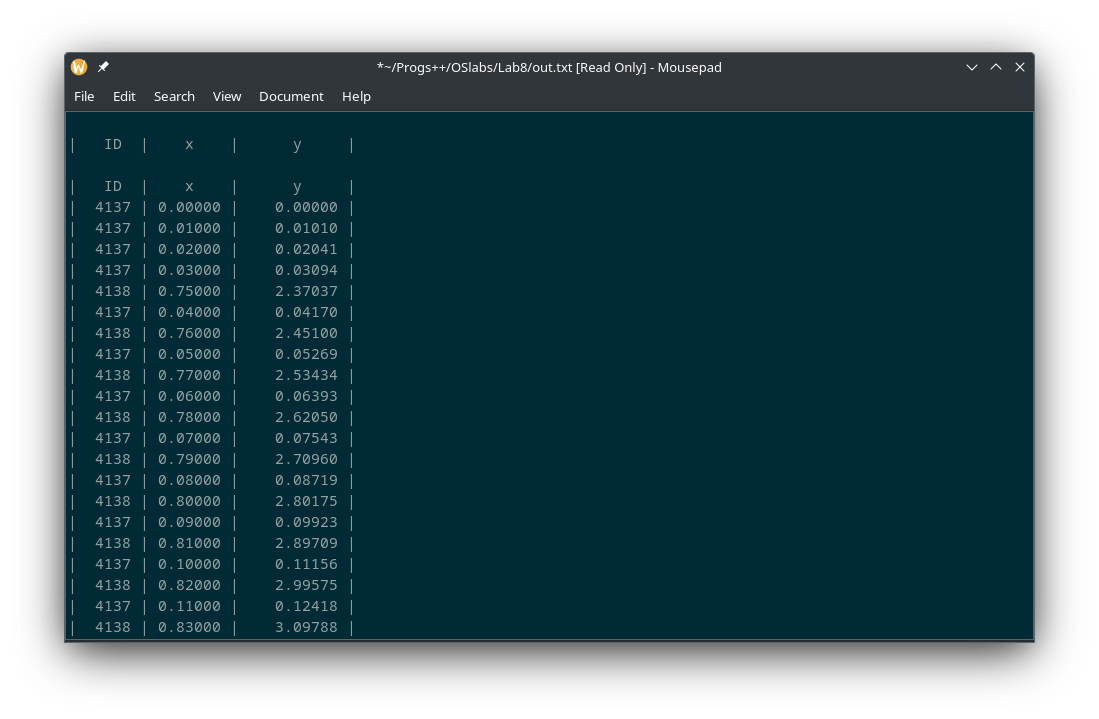
\includegraphics[width=0.90\textwidth]{linux_txt}
    \caption{Вміст файлу}
\end{figure}

\begin{figure}[H]
    \centering
    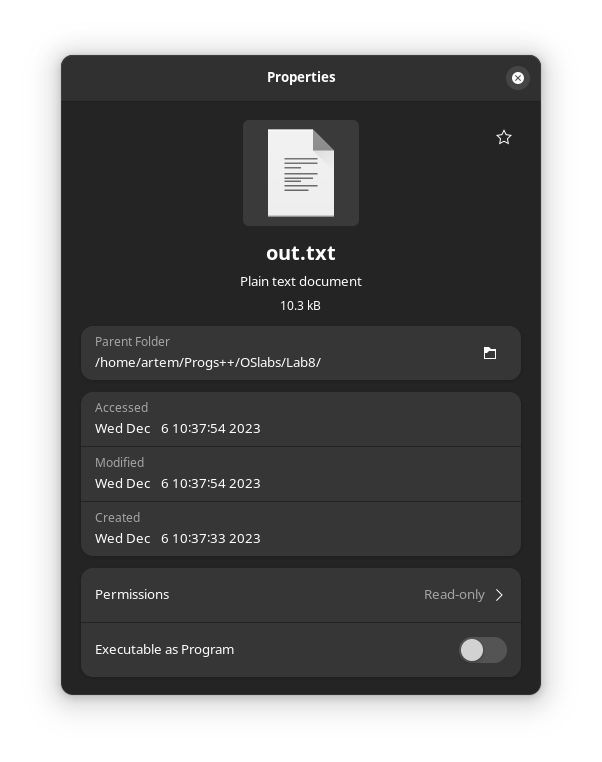
\includegraphics[width=0.90\textwidth]{linux_prop}
    \caption{Властивості файлу}
\end{figure}

\subsection*{Windows}

\begin{figure}[H]
    \centering
    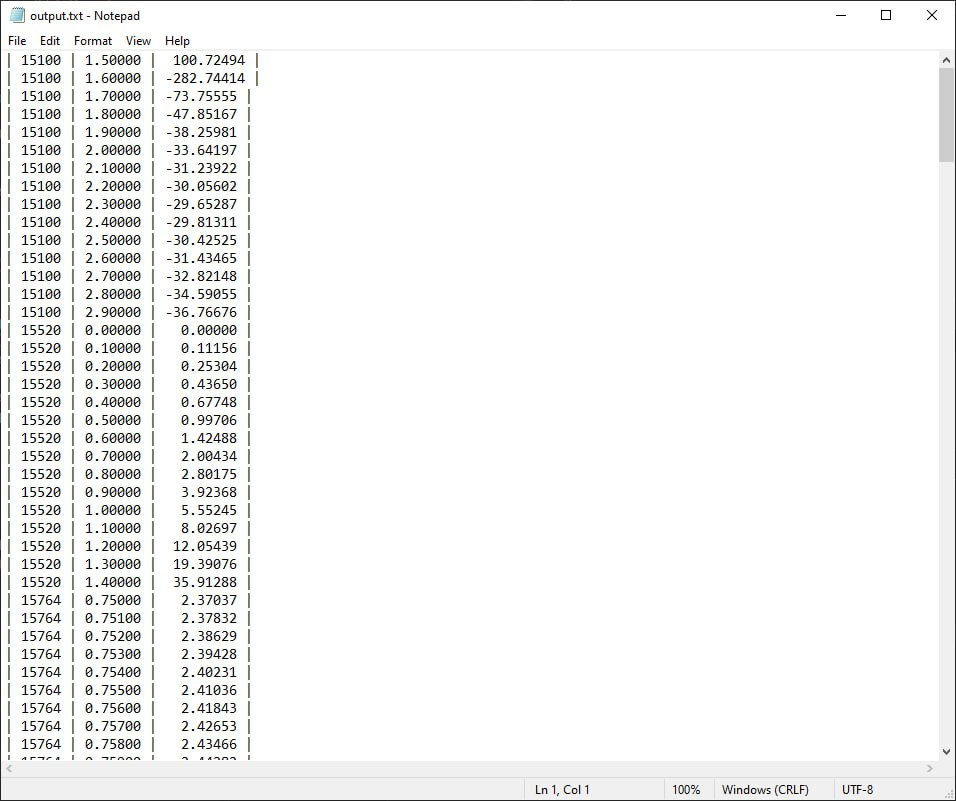
\includegraphics[width=0.90\textwidth]{win_txt}
    \caption{Вміст файлу}
\end{figure}

\begin{figure}[H]
    \centering
    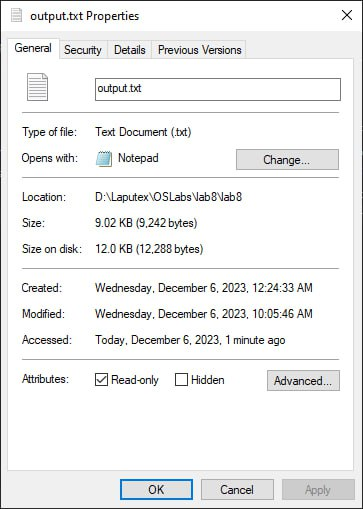
\includegraphics[width=0.90\textwidth]{win_prop}
    \caption{Властивості файлу}
\end{figure}

\textbf{Висновок:}
Я навчився створювати файли і керувати їхніми властивостями в Linux та Windows.
 \end{document}
